%%%%%%%%%%%%%%%%%%%%%%%%%%%%%%%%%%%%%%%%%
% Beamer Presentation
% LaTeX Template
% Version 1.0 (10/11/12)
%
% This template has been downloaded from:
% http://www.LaTeXTemplates.com
%
% License:
% CC BY-NC-SA 3.0 (http://creativecommons.org/licenses/by-nc-sa/3.0/)
%
%%%%%%%%%%%%%%%%%%%%%%%%%%%%%%%%%%%%%%%%%

%----------------------------------------------------------------------------------------
%	PACKAGES AND THEMES
%----------------------------------------------------------------------------------------

\documentclass{beamer}

\mode<presentation> {

% The Beamer class comes with a number of default slide themes
% which change the colors and layouts of slides. Below this is a list
% of all the themes, uncomment each in turn to see what they look like.

%\usetheme{default}
%\usetheme{AnnArbor}
%\usetheme{Antibes}
%\usetheme{Bergen}
%\usetheme{Berkeley}
%\usetheme{Berlin}
%\usetheme{Boadilla}
%\usetheme{CambridgeUS}
%\usetheme{Copenhagen}
%\usetheme{Darmstadt}
%\usetheme{Dresden}
%\usetheme{Frankfurt}
%\usetheme{Goettingen}
%\usetheme{Hannover}
%\usetheme{Ilmenau}
%\usetheme{JuanLesPins}
%\usetheme{Luebeck}
\usetheme{Madrid}
%\usetheme{Malmoe}
%\usetheme{Marburg}
%\usetheme{Montpellier}
%\usetheme{PaloAlto}
%\usetheme{Pittsburgh}
%\usetheme{Rochester}
%\usetheme{Singapore}
%\usetheme{Szeged}
%\usetheme{Warsaw}

% As well as themes, the Beamer class has a number of color themes
% for any slide theme. Uncomment each of these in turn to see how it
% changes the colors of your current slide theme.

%\usecolortheme{albatross}
%\usecolortheme{beaver}
%\usecolortheme{beetle}
%\usecolortheme{crane}
%\usecolortheme{dolphin}
%\usecolortheme{dove}
%\usecolortheme{fly}
%\usecolortheme{lily}
%\usecolortheme{orchid}
%\usecolortheme{rose}
%\usecolortheme{seagull}
%\usecolortheme{seahorse}
%usecolortheme{whale}
%\usecolortheme{wolverine}

%\setbeamertemplate{footline} % To remove the footer line in all slides uncomment this line
%\setbeamertemplate{footline}[page number] % To replace the footer line in all slides with a simple slide count uncomment this line

%\setbeamertemplate{navigation symbols}{} % To remove the navigation symbols from the bottom of all slides uncomment this line
}

\usepackage{graphicx} % Allows including images
\usepackage{booktabs} % Allows the use of \toprule, \midrule and \bottomrule in tables
\usepackage{amsmath}
%----------------------------------------------------------------------------------------
%	TITLE PAGE
%----------------------------------------------------------------------------------------

\title[LLM]{Lifetime Limited Memory} % The short title appears at the bottom of every slide, the full title is only on the title page

\author{J. Matt Maierhofer} % Your name
\institute[CU] % Your institution as it will appear on the bottom of every slide, may be shorthand to save space
{
University of Colorado \\ % Your institution for the title page
\medskip
\textit{} % Your email address
}
\date{\today} % Date, can be changed to a custom date

\begin{document}

\begin{frame}
\titlepage % Print the title page as the first slide
\end{frame}

\begin{frame}
\frametitle{Overview} % Table of contents slide, comment this block out to remove it
\tableofcontents % Throughout your presentation, if you choose to use \section{} and \subsection{} commands, these will automatically be printed on this slide as an overview of your presentation
\end{frame}

%----------------------------------------------------------------------------------------
%	PRESENTATION SLIDES
%----------------------------------------------------------------------------------------

%------------------------------------------------
\section{Introduction} % Sections can be created in order to organize your presentation into discrete blocks, all sections and subsections are automatically printed in the table of contents as an overview of the talk
%------------------------------------------------

%\subsection{Subsection Example} % A subsection can be created just before a set of slides with a common theme to further break down your presentation into chunks

\begin{frame}
\frametitle{Motivation}
\begin{itemize}
\item Event sequence data finds itself in many modern problems
\begin{itemize}
    \item Shopping History
    \item Call Logs
    \item User Behavior
\end{itemize}
\item Temporal aspect of data not specifically addressed by LSTM's structure
\item Event Sequences occur at variety of timescales with varying levels of memory decay
\end{itemize}
\end{frame}

\begin{frame}{Event Sequence Data}
    \begin{figure}
    \centering
    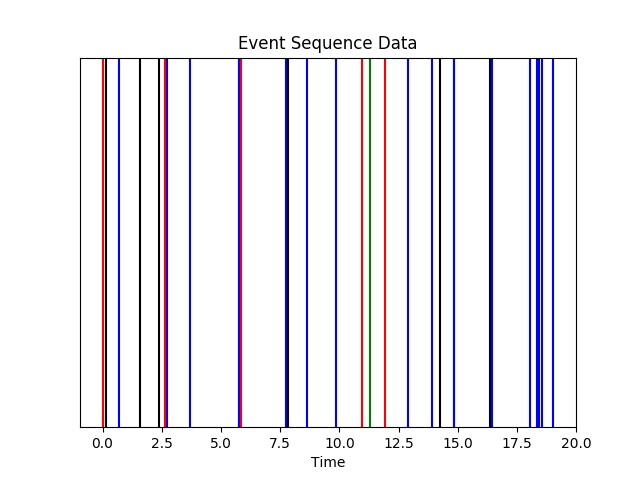
\includegraphics[width=0.6\textwidth]{figures/Event_Sequence.png}
    \caption{Event Sequence Data}
    \label{fig:Event_seq}
    An example of an event sequence with 4 different event types
    
\end{figure}
\end{frame}
\begin{frame}{Neural Networks}
    \begin{itemize}
        \item In the vanilla case, sequence of linear operations followed by activation functions
        \item Parameters of the linear operations are allowed to vary
        \item It has been shown that a single layer neural network is capable of approximating any discrimination task/function given a large enough finite number of neurons (although provides no guarantee about the ability to learn the parameters given an algorithm)\cite{app}
        \item Parameters learned via gradient descent type algorithms
    \end{itemize}
\end{frame}
\begin{frame}{Neural Network Diagram}
    \begin{figure}
    \centering
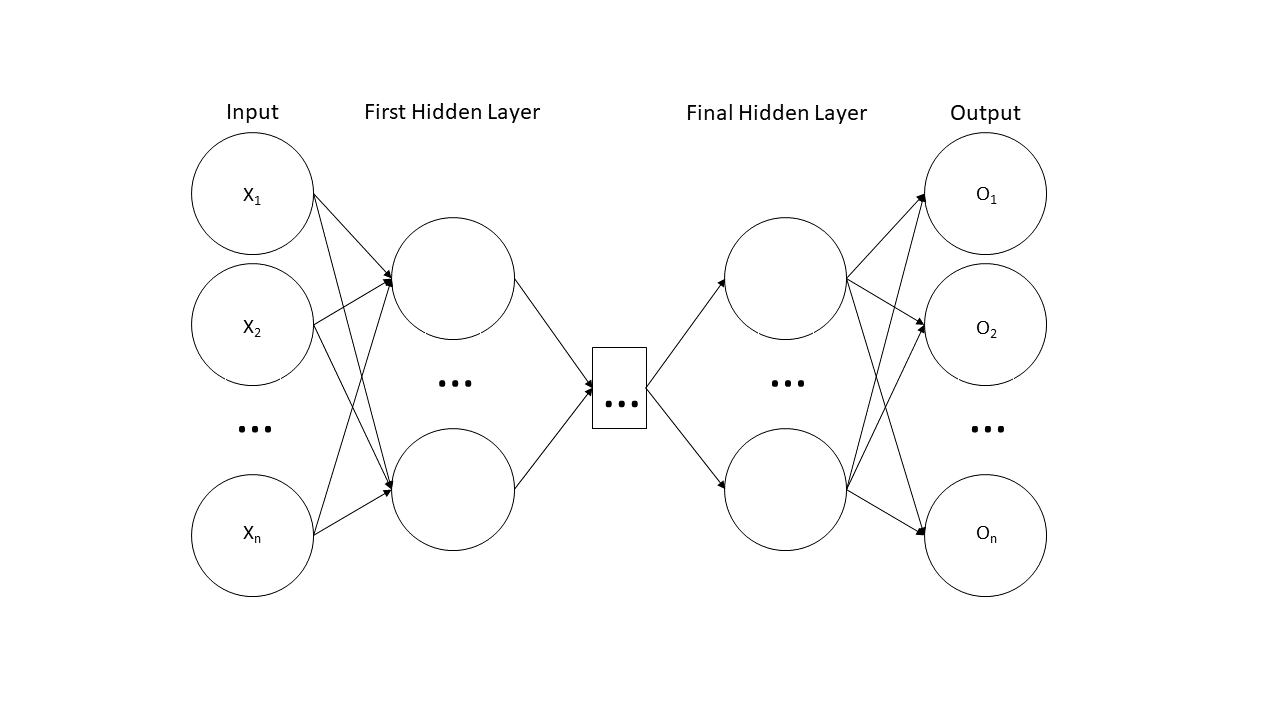
\includegraphics[width=0.8\textwidth]{figures/NN.png}
    \caption{Neural Network}
    \label{fig:NN}
    Diagram of a vanilla neural network
\end{figure}
\end{frame}
\begin{frame}{Recurrent Neural Networks}
\begin{itemize}
    \item Introduces notion of memory to neural network
    \item Formulated to work on sequences of data
    \item In vanilla case, passes previous output of network into next input
    \item Doesn't include ability to pass on long term memory in vanilla 
\end{itemize}
    
\end{frame}
\begin{frame}{RNN Diagram}
    \begin{figure}
    \centering
    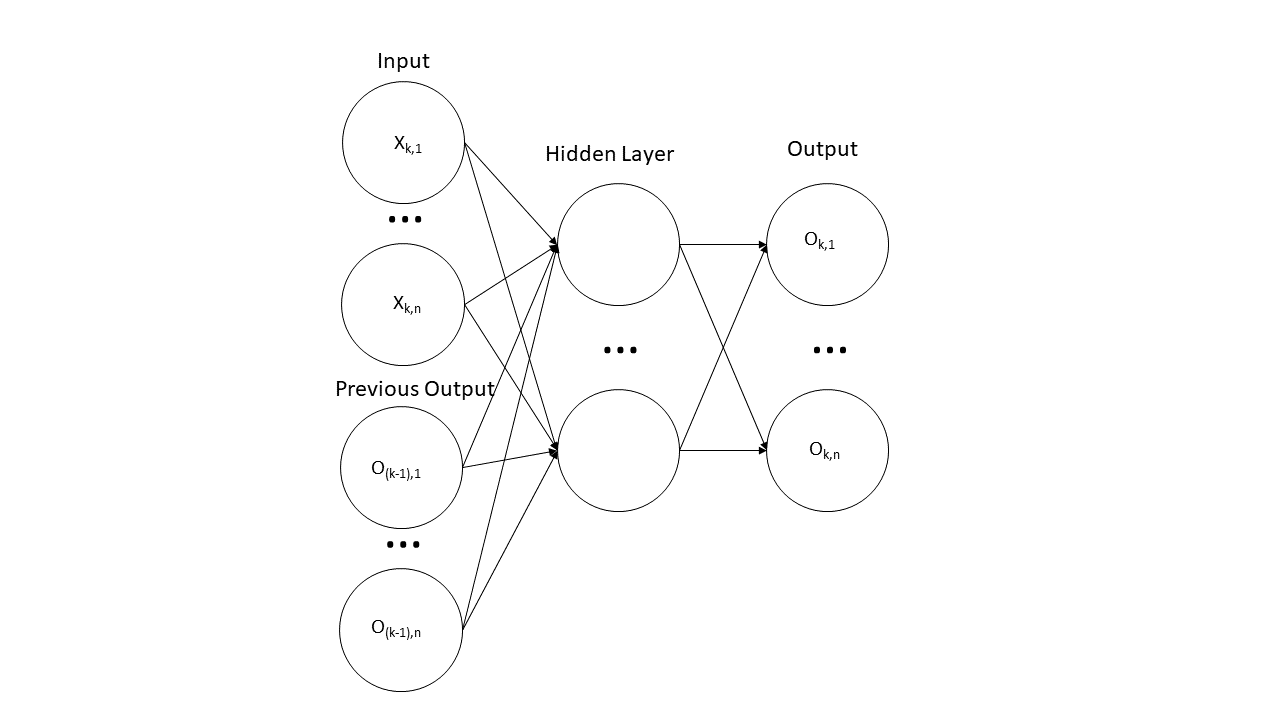
\includegraphics[width=0.8\textwidth]{figures/RNN.png}
    \caption{Recurrent Neural Network}
    \label{fig:rnn}
    Diagram of a vanilla recurrent neural network
\end{figure}
\end{frame}

\begin{frame}{Long Short-Term Memory}
\begin{itemize}
    \item Introduced in 1997\cite{LSTM}
    \item Solves memory problem in RNNs by introducing memory traces across all sequence (an output independent of the classification)
    \item Parameters determine how memory traces are forgotten and learned, as well as the more traditional uses from neural networks.
\end{itemize}
    
\end{frame}
%------------------------------------------------


\begin{frame}
\frametitle{References}
\bibliographystyle{alpha}
\bibliography{refs}
\end{frame}

%------------------------------------------------
\begin{frame}{Acknowledgements}
\begin{itemize}
    \item Faculty Advisors: Michael Mozer and Stephen Becker
\item Continuing Work done by Denis Kazakov
\item Funding Provided by National Science Foundations EXTREEMS Grant,   DMS 1407340 through Anne Dougherty.
\end{itemize}
\end{frame}
\begin{frame}
\begin{center}

\includegraphics[width=0.6\textwidth]{SkoBuffs.jpg}
\end{center}
\end{frame}

%----------------------------------------------------------------------------------------

\end{document}